% !TeX spellcheck = fr_FR
\thispagestyle{noheader}
\chapter*{Résumé} % No (numbered) toc entry with *
\addcontentsline{toc}{chapter}{Résumé} % Adding toc entry
\thispagestyle{noheader}

Depuis l'antiquité à nos jours, les cartes sont le reflet des premières formes de données récoltées par l'Homme.
La cartographie a aidé l'humanité à définir des chemins à travers le monde et à naviguer.
Cependant avec les fortes avancées technologiques des dernières décennies, les données récoltées ont augmenté massivement et notablement dans la cartographie avec les données LIDAR. Elles représentent un nuage de point dense qui sont actuellement une des informations collectées des plus massives.
Elles sont utilisées dans l'étude topographique de régions, dans les géosciences, dans la science environnementale ou bien encore elles viennent en aide au guidage automatique de véhicule terrestre. Un problème fréquent lié à ces données est le traitement réalisé avant leurs utilisations dans des applications, qui est souvent nécessaire afin de filtrer tout ce qui ne présente aucune utilité et pourrait même fausser les résultats.
Il reste cependant difficile de les traiter manuellement due à la quantité de données importante. Pour ce faire, des méthodes analytiques sont employées afin d'accélérer ce processus au travers de systèmes automatisés.
Un autre problème présent est leurs utilisations pour reconstruire des surfaces. Les méthodes automatisées n'étant pas à 100\% fiables, il est nécessaire de vérifier la cohérence des données ainsi que la qualité des maillages produits.
Un objectif supplémentaire est de réduire leurs empreintes volumiques sur les moyens de stockage. Ce travail se focalise sur principalement sur la création d'outils de traitement de données LIDAR et l'affichage de ces données au travers d'un client web.


\begin{figure}[htbp!]
    \centering
    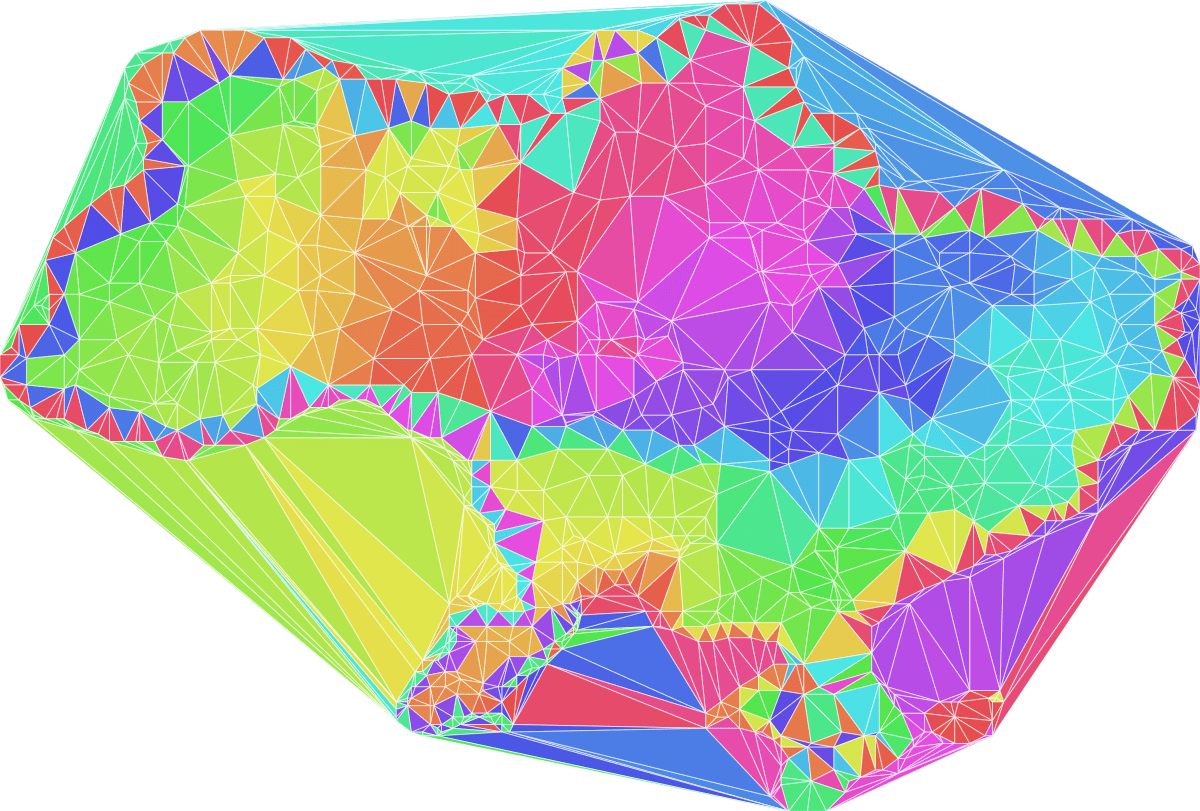
\includegraphics[width=0.5\linewidth]{figures/delaunator.png}
    \caption{Maillage résultant d'une triangulation de Delaunay. Source : tiré de \href{https://github.com/mapbox/delaunator}{https://github.com/mapbox/delaunator}}
    \label{fig:my_label}
\end{figure}